% 矢量内积
% 线性代数|几何矢量|内积|dot product|点积|标量积|scalar product|内积|inner product|正交|归一化|正交归一基|交换律|分配律

% 这里只介绍几何矢量及对应的直角坐标列矢量
\pentry{几何矢量\upref{GVec}}

\subsection{几何定义}
我们先来看内积的几何定义. 注意该定义不需要任何坐标系的概念.
\begin{figure}[th]
\centering
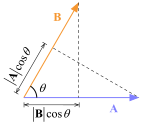
\includegraphics[width=5cm]{./figures/Dot1.pdf}
\caption{内积的几何定义}\label{Dot_fig1}
\end{figure}

如\autoref{Dot_fig1}, 两个几何矢量的\textbf{内积(inner product)}\footnote{也叫\textbf{点积} 或 \textbf{点乘},\textbf{标量积(scalar product)}}就是把它们的模长相乘,再乘以它们的夹角的余弦值.即
\begin{equation}\label{Dot_eq1}
\bvec A \vdot \bvec B = \abs{\bvec A} \abs{\bvec B} \cos\theta 
\end{equation}

其中 $\theta$ 是两个矢量的夹角. 注意两个矢量内积得到的是一个标量. 几何定义中(\autoref{Dot_fig1}),既可以把内积理解为 $\bvec A$ 投影在 $\bvec B$ 上的模长乘以 $\bvec B$ 的模长,也可以理解为 $\bvec B$ 投影在 $\bvec A$ 上的模长乘以 $\bvec A$ 的模长\footnote{在这种理解下,若量矢量的夹角为钝角,投影长度取负值}.可见当两矢量模长不变时,若方向相同,内积取最大值 $\abs{\bvec A}\abs{\bvec B}$;若方向相反,内积取最小值 $-\abs{\bvec A}\abs{\bvec B}$;若相互垂直,则内积为 0.

我们说两个内积为 0 的矢量互相垂直, 或者说\textbf{正交}. 几何矢量与自身内积可得该矢量模长的平方. 单位矢量与自己的内积等于 1. 把一个矢量除以自身模长得到同方向单位矢量的过程叫做矢量的\textbf{归一化}.

\subsection{内积的性质}

\begin{enumerate}
\item \textbf{交换律 \footnote{由\autoref{Dot_eq1} 易证}}
\begin{equation}\label{Dot_eq2}
\bvec A \vdot \bvec B = \bvec B \vdot \bvec A
\end{equation}

\item \textbf{分配律 \footnote{证明见词条最后.}}
\begin{equation}\label{Dot_eq3}
\bvec A \vdot (\bvec B + \bvec C) = \bvec A \vdot \bvec B + \bvec A \vdot \bvec C
\end{equation}
\end{enumerate}

注意内积不满足结合律,即
\begin{equation}
(\bvec A \vdot \bvec B) \bvec C \ne  \bvec A (\bvec B \vdot \bvec C)
\end{equation}
前者是 $\bvec C$ 方向的矢量,后者是 $\bvec A$ 方向的矢量,显然不相等.

\subsection{内积的坐标运算}
\pentry{正交归一基\upref{OrNrB}}
若已知 $\bvec A, \bvec B$ 在平面直角坐标系 $xy$ 中坐标分别为 $(A_x, A_y)$ 和  $(B_x, B_y)$,那么如何用坐标表示内积运算的结果呢? 先用正交归一基\upref{OrNrB} 将两矢量展开 %未完成,矢量空间里面要介绍基底及坐标的唯一性.
\begin{equation}
\bvec A = A_x \,\uvec x + A_y \,\uvec y \qquad \bvec B = B_x \,\uvec x + B_y \,\uvec y
\end{equation}
所以
\begin{equation}
\bvec A \vdot \bvec B = (A_x \,\uvec x + A_y \,\uvec y) \vdot (B_x \,\uvec x + B_y \,\uvec y)
\end{equation}
根据分配律\autoref{Dot_eq3},我们可以把两个括号拆开,变为 4 个内积之和. 
\begin{equation}
\bvec A \vdot \bvec B = A_x B_x \,\uvec x \vdot \uvec x + A_y B_y \,\uvec y \vdot \uvec y + A_x B_y \,\uvec x \vdot \uvec y + A_y B_x \,\uvec y \vdot \uvec x
\end{equation}
其中 $\uvec x \vdot \uvec y = \uvec y \vdot \uvec x = 0$ (相互垂直), 而 $\uvec x \vdot \uvec x = \uvec y \vdot \uvec y = 1$ (相互平行且模长都为1). 所以最后结果为
\begin{equation}
\bvec A \vdot \bvec B = A_x B_x + A_y B_y
\end{equation}
同理,可以在三维直角坐标系 $xyz$ 中把内积结果用坐标表示
\begin{equation}
\bvec A \vdot \bvec B = A_x B_x + A_y B_y + A_z B_z	
\end{equation}
注意内积的代数定义也可以拓展到更高维的情况甚至复数的情况, 即对于复数域的 $u_1, u_2, \dots, u_N$ 和 $v_1, v_2, \dots, v_N$,
\begin{equation}
\bvec u \vdot \bvec v = \sum_k u_k v_k
\end{equation}

注意虽然上式中的坐标取决于正交归一基底的选取, 但内积的结果却与基底的选取无关. 这是因为内积的几何定义是两个几何矢量间的几何性质, 与基底无关.

\begin{figure}[ht]
\centering
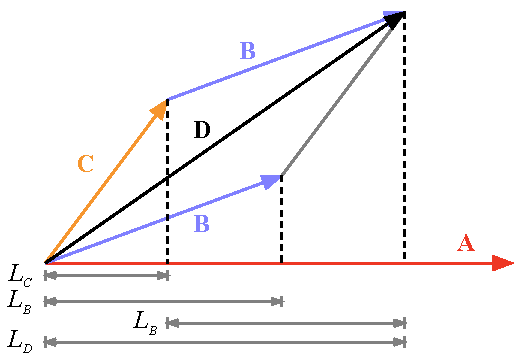
\includegraphics[width=8cm]{./figures/Dot2.pdf}
\caption{内积分配律的证明} \label{Dot_fig2}
\end{figure}

\subsection{证明内积的分配律}

如\autoref{Dot_fig2}, 令 $\bvec D \equiv \bvec B + \bvec C$, 把 $\bvec A \vdot \bvec B$,  $\bvec A \vdot \bvec C$,  $\bvec A \vdot \bvec D$ 分别用几何定义理解为 $\bvec B$,  $\bvec C$,  $\bvec D$ 在 $\bvec A$ 上的投影乘 $\abs{\bvec A}$, 且令投影长度分别为 $L_B, L_C, L_D$. 那么要证明 $\bvec A \vdot (\bvec B + \bvec C) = \bvec A \vdot \bvec D = \bvec A \vdot \bvec B + \bvec A \vdot \bvec C$, 只需证明 $L_D = L_B + L_C$ 即可.现在把 $\bvec B$ 平移使其起点与 $\bvec C$ 的终点对接(投影长度不变). 从图中立即得出 $L_D = L_B + L_C$.  








